%Template v.1.0: Taylor Arnold and Simon Gabay, december 2025
% CECI EST UN FICHIER DE MODÈLE LATEX POUR LES ARTICLES INCLUS DANS
% *Anthology of Computers and the Humanities*. AJOUTEZ L'OPTION
% 'final' LORS DE LA CRÉATION DE LA VERSION FINALE DE L'ARTICLE. 
% NE PAS modifier la classe du document
\documentclass[final, fra]{anthology-ch}     % pour la version finale
%\documentclass[fra, custom]{anthology-ch}      % pour la soumission

% CHARGER LES PACKAGES LaTeX
\usepackage{booktabs}
\usepackage{graphicx}

% AJOUTEZ vos propres packages avec \usepackage{}

% TITRE DE LA SOUMISSION
% Remplacez ceci par le titre de votre soumission
\title{Les \textit{embeddings}, nouvel outil d’une histoire numérique des grands corpus de presse?}

% INFORMATIONS SUR LES AUTEURS ET LES AFFILIATIONS
% Pour chaque auteur, utilisez une nouvelle commande \author, avec
% les numéros entre crochets indiquant les affiliations correspondantes
% (section suivante) et l'ORCID-ID pour chaque auteur.  
\author[1]{Arthur Michelet}[
  orcid=0009-0006-4593-6402,
  email=arthur.michelet@unil.ch
]

\author[1]{Martin Grandjean}[
  orcid=0000-0003-3184-3943,
  email=martin.grandjean@unil.ch
]

% Il doit y avoir un appel à \affiliation pour chaque affiliation des auteurs.
% Plusieurs affiliations peuvent être attribuées à un auteur
% et une affiliation peut être attribuée à plusieurs auteurs. 
\affiliation{1}{Université de Lausanne}

% MOTS-CLÉS
% Fournissez un ou plusieurs mots-clés séparés par des virgules
% en utilisant les commandes suivantes
\keywords[fra]{Histoire, histoire économique, histoire des médias, relations publiques, traitement automatique des langues, embeddings, humanités numériques, humanités computationnelles, visualisation de données}
\keywords[eng]{History, economic history, media history, public relations, natural language processing, embeddings, digital humanities, computational humanities, data visualization}

% MÉTADONNÉES DE LA PUBLICATION
% Ces champs seront remplis lors de la publication ; 
% ils peuvent être laissés par défaut lors de la soumission
\pubyear{2026}
\pubvolume{4}
\pagestart{175}
\pageend{181}
\paperorder{21}
\conferencename{Actes de la Conférence Humanistica}
\conferenceeditors{Serena Crespi, Simon Gabay, Martin Grandjean, Ariane Pinche, Marie Puren et Léa Saint-Raymond}
\doi{10.63744/R2LLVRsBeNuI}
\customhead{}

\addbibresource{references.bib}

%%%%%%%%%%%%%%%%%%%%%%%%%%%%%%%%%%%%%%%%%%%%%%%%%%%%%%%%%%%%%%%%%%%%%%%%%%%
% DÉBUT DU TEXTE
\begin{document}

\maketitle

\begin{abstract}
This research focuses on the development of a procedure for analyzing very large corpora of news articles. It discusses the cross-analysis of archival sources and news articles using text embeddings within a notebook designed for historians and students.
\end{abstract}

\section{Introduction} 
En raison de leur nature massive et hautement standardisée, et plus récemment en raison d'un intense effort de numérisation, les archives de presse constituent des sources d'intérêt majeur pour l'histoire numérique, un véritable « Eldorado » à explorer \cite{Bunout2023b}. Au cours de la dernière décennie, l'intérêt pour ces corpus a donné lieu à des projets interdisciplinaires à grande échelle, tels que \href{http://www.numapresse.org}{Numapresse (http://www.numapresse.org)}, \href{https://viraltexts.org}{ViralTexts (https://viraltexts.org)}, \href{https://www.newseye.eu/}{NewsEye (https://www.newseye.eu/)} ou \href{https://impresso-project.ch/}{Impresso (https://impresso-project.ch/)}. Il s'agit là d'un terrain particulièrement fertile pour l'innovation, qu'il s'agisse du traitement et de l'enrichissement de ces données, de leur analyse à l'aide de toute une gamme d'outils de lecture distante, ou de leur mise à disposition du grand public via des interfaces en ligne \cite{Ehrmann2023e}.

Nous développons, questionnons et critiquons une approche de \textit{distant reading} \cite{Underwood2017} basée sur les \textit{text embeddings}, une méthode qui consiste à calculer la proximité sémantique des articles de presse dans un espace multidimensionnel. Cette approche vise à développer un pipeline d’analyse qui consiste à calculer la proximité de milliers d’articles de la presse suisse (francophones et germanophones principalement) et de la comparer à des sources historiques externes pour discuter de la pertinence des clusters détectés, dans notre cas des documents permettant d’étudier l’activité de communication des banques suisses au XXe siècle. Au-delà d’un outil d’analyse destiné uniquement aux membres du projet, le \textit{notebook} ainsi créé \cite{Michelet2026b} a pour vocation de rejoindre un \textit{datalab} public à disposition des chercheuses et chercheurs en histoire numérique des médias et être utilisé dans le cadre de plusieurs enseignements de Master dans les universités des porteurs du projet. Lier une étude de cas à ce questionnement épistémologique et pédagogique nous permet d’éviter les écueils d’une approche trop théorique et de fonder ces réflexions sur des problématiques historiques concrètes.

\section{Les \textit{text embeddings} au service d’une analyse des corpus de presse}
Récente addition à la boîte à outils du \textit{Natural Language Processing} (NLP), les \textit{embeddings} (ou “plongement sémantique”) complètent des approches d’analyse de grands corpus de presse déjà existantes comme le \textit{topic model} \cite{Murugaraj2025a} en permettant de mesurer la distance entre plusieurs textes, promettant de “cartographier la signification ou le contenu des phrases et documents sous forme de représentations vectorielles” \cite{Opitz2025d}. Une réduction de la dimensionnalité de cette distance, mesure de similarité sémantique entre ces textes qui s’exprime dans un espace de vecteurs à plusieurs centaines voire milliers de dimensions, permet de produire une représentation graphique synthétique qui aplatit la complexité sémantique du corpus choisi sous la forme d’une carte (UMAP) de clusters de textes.

Au vu de la nature sérielle des grands corpus de presse numérisés, il semble qu’une telle méthode permet de s’inscrire efficacement dans une démarche de \textit{distant reading}. Les cartes produites permettent en effet une première évaluation de la nature du corpus, les clusters étant susceptibles de permettre une classification thématique des différents articles, soit pour comprendre la couverture médiatique globale de l’actualité par la presse pendant une période donnée (Figure~\ref{fig:figure1}), soit, à plus petite échelle, pour appréhender les différents discours à l’intérieur d’une actualité particulière.

\begin{figure}[t!]
  \centering
  
\includegraphics[width=1\linewidth]{figure1.png}
  \caption{UMAP (sous la forme d’un \textit{7-nearest neighbors network}) de tous les articles du Journal de Genève du 1er au 10 mars 1932. Chaque nœud est un article, deux nœuds sont connectés s’ils font partie des 7 textes les plus proches l’un de l’autre. Exemple produit avec un \textit{notebook} dédié à l’analyse de réseaux de textes \cite{Jacomy2025} et visualisé avec Gephi Lite \cite{Girard2025}.}
  \label{fig:figure1}
\end{figure}

L’appropriation de telles méthodes de la linguistique computationnelle par les sciences historiques pose une série de questions :
\begin{itemize}
    \item Dans quels cas ce type d’approche est-elle justifiée ?
    \item Correspond-elle à ce que d’autres méthodes de classification proposent déjà pour l’exploration de grands corpus de textes ? Dans ce cas, est-ce que la redondance permet de déterminer des classes/clusters robustes ou au contraire rend-elle cette approche superflue ? Si ce n’est pas le cas, est-ce que les différences montrent quelque chose de qualitativement probant, des cas d’usages privilégiés pour les unes ou les autres, ou cela met-il au contraire en évidence un manque de fiabilité de cette nouvelle méthode ?
    \item Apporte-t-elle des résultats plus probants lorsque le corpus de presse est très vaste et généraliste (auquel cas elle sert à comprendre une sorte de “panorama” global de la couverture médiatique) ou quand les articles ont été soigneusement sélectionnés autour d’un thème ou d’une période resserrée (auquel cas il s’agit avant tout de tracer les différentes manières de couvrir un événement) ?
    \item Dans quelles conditions est-il possible de faire une analyse conjointe d’un corpus d’articles de presse et d’un corpus d’autres documents historiques ? La réduction de la dimensionnalité permet-elle valablement de comparer les représentations vectorielles de ces deux types de textes ensemble ? Cette comparaison permet-elle d’enrichir l’étude de grands corpus médiatiques ou ne fait-elle que de montrer des évidences ?
\end{itemize}

\section{Sources et données : actualité bancaire et relations publiques des banques suisses}

Afin d'explorer la dimension comparative des \textit{embdeddings}, notre recherche utilise deux corpus distincts qui permettent d’aborder une étude de cas sur l’histoire de la communication des banques suisses. Tout d’abord, elle repose sur les collections de presse numérisées rendues accessibles par le projet Impresso sur \href{https://impresso-project.ch/app/}{sa plateforme (https://impresso-project.ch/app/)} et \href{https://impresso-project.ch/datalab/}{\textit{via} son API (https://impresso-project.ch/datalab/)}. S’ajoutent ensuite des sources tirées de recherches dans les archives de l'Association suisse des banquiers (ASB), conservées aux Archives économiques suisses (Bâle).

L’actualité bancaire offre un objet d’étude particulièrement adapté à l’exploration de grands corpus de presse par \textit{embeddings}, ainsi qu’à la comparaison, par la mesure de similarité d’\textit{embeddings}, de ces corpus et de sources externes. Les banques sont en effet présentes dans la presse quotidiennement et sous des formes qui vont bien au-delà des articles : leur activité est couverte par des dépêches financières, diverses informations tabulaires, de la publicité, etc. L’actualité bancaire se retrouve donc sur un large spectre de la surface éditoriale d’un journal.

\begin{figure}[t!]
  \centering
  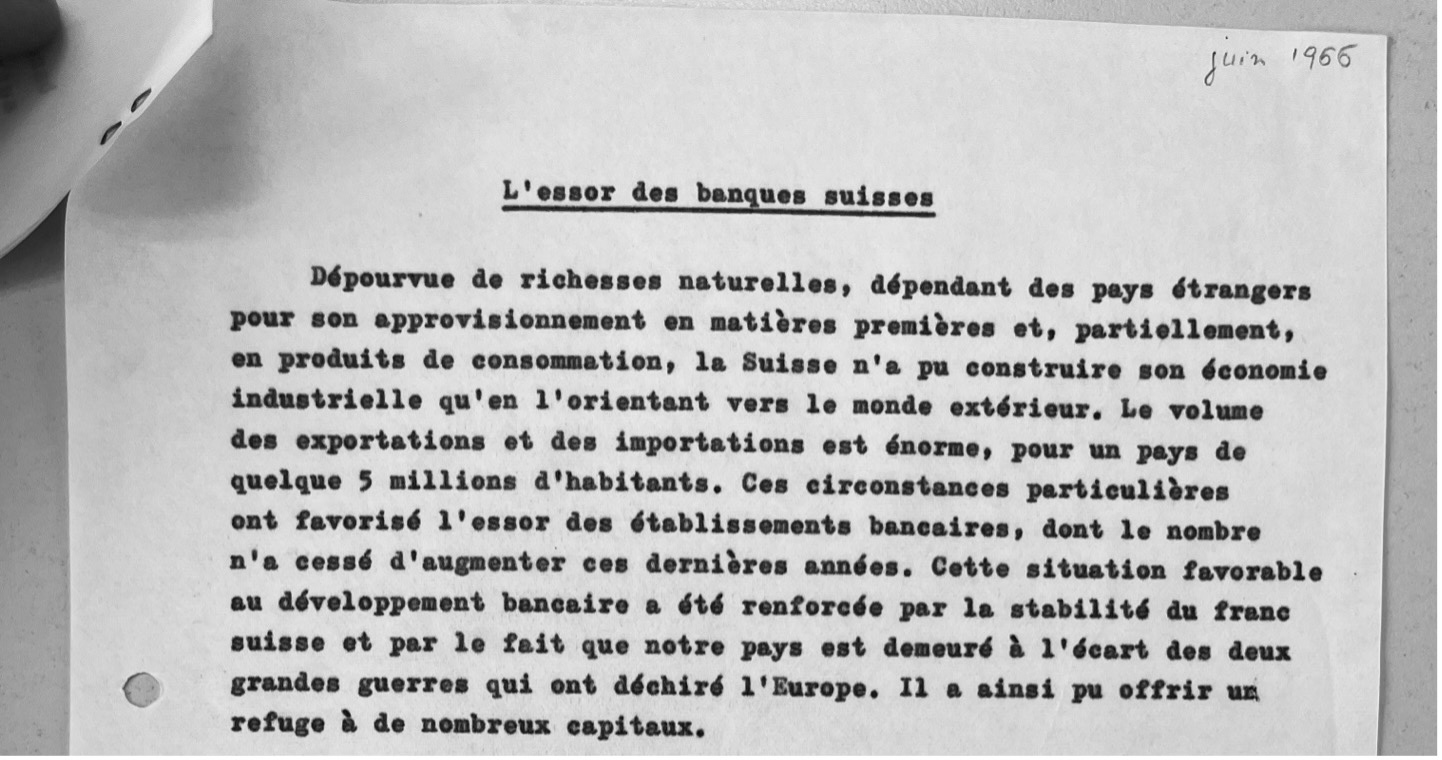
\includegraphics[width=1\linewidth]{essorebanquessuisses.jpg}
  \caption{Extrait d’un texte rédigé par le président de la commission de relations publiques de l’ASB (Hans Bauer), destiné à être publié dans la revue britannique Statist. Ce texte encapsule un certain type de discours sur les banques suisses typique des relations publiques de l’ASB que l’on retrouve généralement dans tout contenu médiatique que cette association produit. Source : Archives économiques suisses (Bâle), PA 650, G 3-0-1160, NF\_0408, 1964/08-1967/05, Hans Bauer (Société de Banque Suisse), “L’essor des banques suisses”, juin 1966.}
  \label{fig:essor}
\end{figure}

En outre, dès la fin des années 1940, les banques cherchent, en Suisse, à influencer collectivement le flux d’information les concernant \cite{Michelet2025e}. S’inscrivant dans une dynamique également observée au Royaume-Uni \cite{Reveley2014b}, l’Association suisse des banquiers — organisation patronale et faîtière \cite{Guex2012a} — établit une commission de relations publiques en 1947 \cite{Michelet2026a}. Celle-ci vise, d’une part, à faire de la “publicité éditoriale”, c’est-à-dire à impulser une couverture médiatique favorable aux banques en cultivant des liens personnels, parfois proches, avec les journalistes, et, d’autre part, à produire directement du contenu médiatique souvent non signé (articles de journaux et de revues, émissions de radio, court-métrages, etc.) ou du contenu publicitaire (encarts, spots TV, etc.). Si l’on peut documenter, par un travail d’archives, la mise en place institutionnelle et la fabrication matérielle des relations publiques de l’ASB, la question de l’efficacité de ce travail demeure, comme souvent dans l’étude des “pratiques d’influence” \cite{Cohen2017b} ou de la “communication persuasive organisée” \cite{Bakir2019b}, difficile à aborder et à évaluer.

Dès lors que les \textit{embeddings} permettent de mesurer la similarité sémantique entre différents textes, on peut se demander s'ils pourraient être mobilisés pour étudier la correspondance entre un contenu de type relations publiques et une couverture médiatique. Une approche \textit{data-driven} de ce type permet-elle d'explorer conjointement les structures sémantiques de l’actualité bancaire et des relations publiques collectives des banques suisses ? Les \textit{embeddings} peuvent-ils répondre à la question de savoir si l’ASB parvient ou non à influencer à une échelle significative la couverture des banques dans la presse suisse ?

 
\section{Développer un \textit{notebook} d’analyse comparée}

Notre démarche s’inscrit dans une volonté de développer des outils d’analyse accessibles et reproductibles. En cela, notre contribution prolonge nos réflexions sur le développement de \textit{notebooks} publics, amenés à être utilisés par des chercheur.euse.s non spécialistes des méthodes d’humanités numériques. Le projet Impresso, dont l’objectif premier était la constitution d’une base de données d’archives de presse, a ainsi lancé à l’automne 2025 un \href{https://impresso-project.ch/datalab/}{datalab (https://impresso-project.ch/datalab/)}. Comportant un comité éditorial, des règles, une évaluation externe ainsi qu’une citabilité, ce site vise à rendre accessible des \textit{notebooks} utilisant les modèles développés au sein du projet tels que la reconnaissance d’agence de presse ou l’analyse de cooccurrence d'entités nommées. Dans cette optique, nous avons fait de l’analyse comparative de deux corpus un \textit{notebook} voué à être rendu publiquement disponible sur le \textit{datalab} d’Impresso.

\begin{figure}[t!]
  \centering
  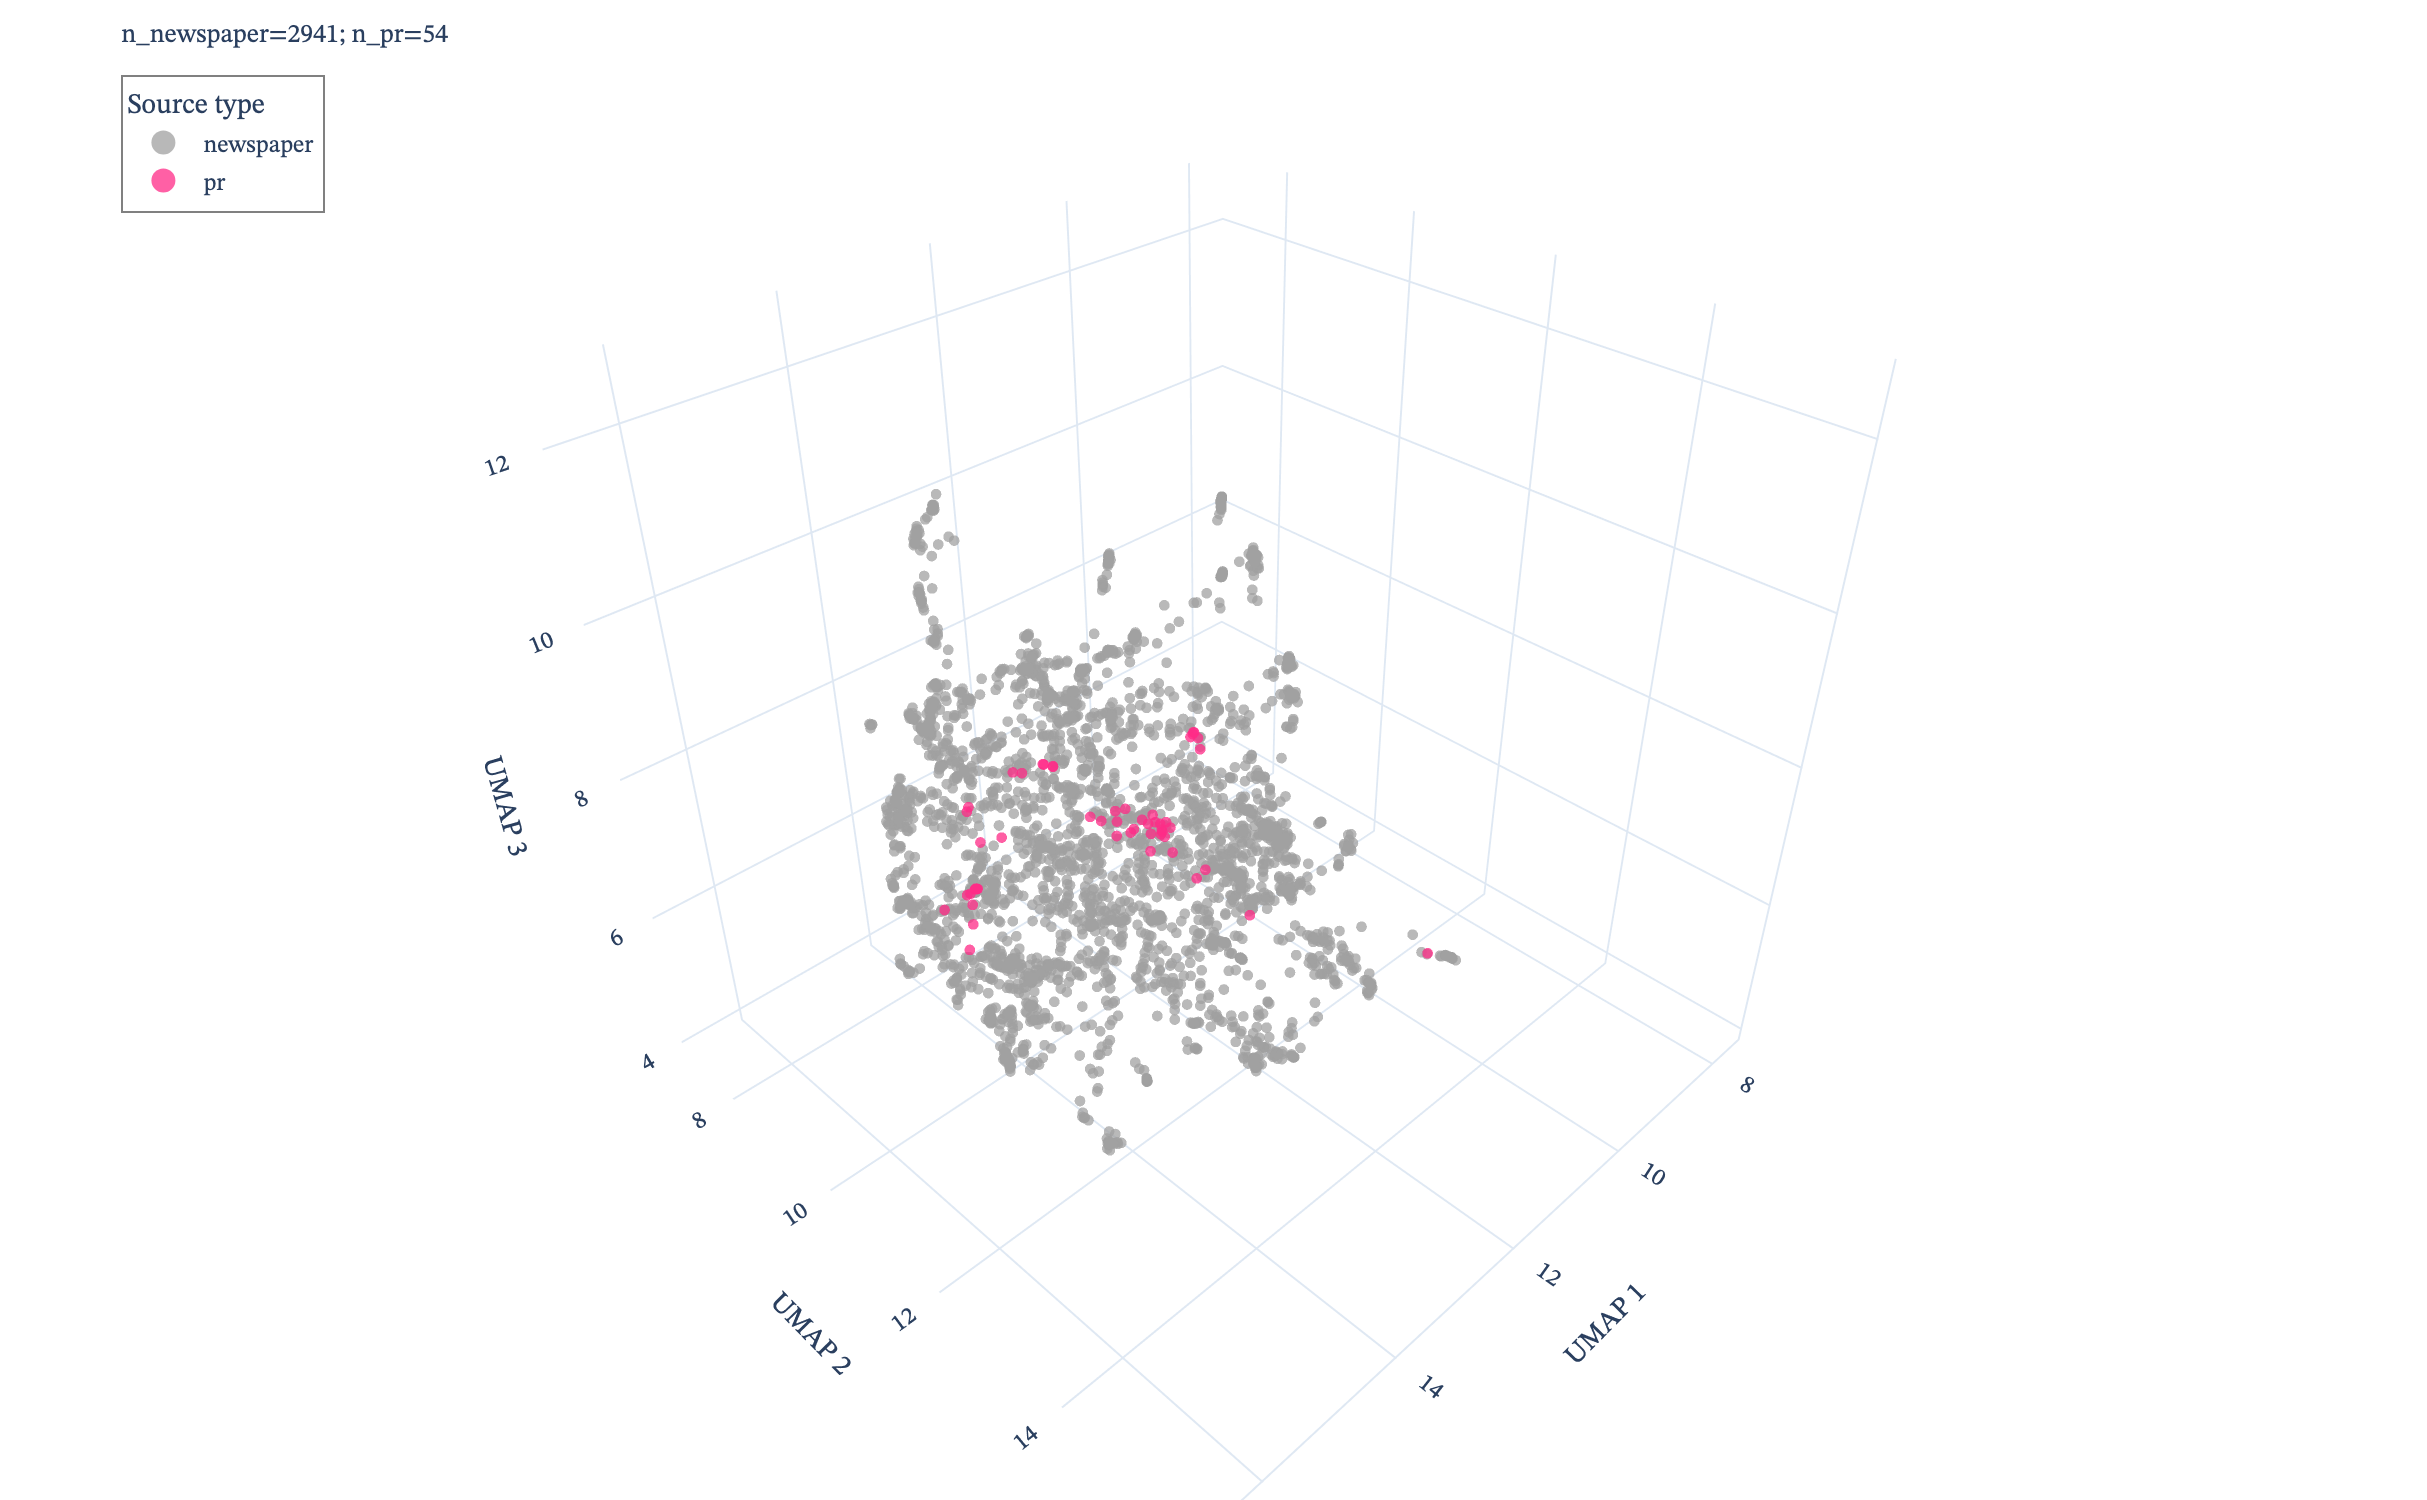
\includegraphics[width=1\linewidth]{cc.png}
  \caption{Exemple d’output du \textit{notebook} \cite{Michelet2026b}: comparaison des \textit{embeddings} de deux corpus. En gris, 2941 articles de presse suisse (français et allemand) publiés entre le 01.01.1950 et le 31.12.1980 mentionnant “Association suisse des banquiers” ou “Schweizerische Bankiervereinigung”. Les articles sont tirés de la plateforme \href{https://impresso-project.ch/app}{Impresso} (\href{https://impresso-project.ch/app/search?sq=CgIYAgpLEAIYByABKiBhc3NvY2lhdGlvbiBzdWlzc2UgZGVzIGJhbnF1aWVycyohc2Nod2VpemVyaXNjaGUgYmFua2llcnZlcmVpbmlndW5nCjIQAhgKKiwxOTUwLTAxLTAxVDAwOjAwOjAwWiBUTyAxOTgwLTEyLTMxVDIzOjU5OjU5Wg==&p=1}{voir la requête complète ici}). En rose, 54 textes (articles, articles payés, communiqués de presse et discours officiels) tirés des archives de l’ASB (Archives économiques suisses, Bâle) et de Leo Schürmann, membre de sa commission de relations publiques (Archives fédérales suisses, Berne), rédigés entre 1950 et 1980.}
  \label{fig:umap3d}
\end{figure}

Le \textit{notebook} \cite{Michelet2026b} a deux objectifs principaux : d’une part, \textit{embed} les textes présents dans deux corpus distincts, c’est-à-dire assigner un vecteur à haute dimension à chaque texte, et, de l’autre, produire une visualisation unique regroupant l’ensemble de ces données. Il se découpe ainsi plus précisément en trois étapes distinctes: l’\textit{embedding} des textes, la réduction des vecteurs à trois dimensions, et la production d’une représentation visuelle pour l'exploration des données. La première phase repose sur les modèles développés par Impresso. Le projet propose une bibliothèque python accessible que nous avons utilisée en passant par son API. Pour l’\textit{embedding} de textes, Impresso utilise le modèle \textit{multilingual General Text Embeddings} (mGTE), ainsi qu’une de ses variantes adaptées aux problèmes d’OCR \cite{Michail2025e}. Le mGTE est très performant tant sur une langue que sur plusieurs \cite{Enevoldsen2025a}, ce qui en fait un modèle idéal pour un corpus multilingue comme le nôtre, qui comprend des textes en allemand, en français et en anglais. En second lieu, nous avons utilisé UMAP pour la compression des vecteurs en trois dimensions. UMAP est en effet très efficace pour réaliser ce genre d’opération en préservant à la fois les relations de voisinage locales et la structure globale des données. Enfin, Plotly a été utilisé pour créer une visualisation interactive, en trois dimensions rendant visible les deux collections (Figure~\ref{fig:umap3d}).

Sachant que le \textit{clustering} des vecteurs indique la proximité sémantique des textes, l’analyse semble tout d'abord mettre en évidence les structures thématiques de chacun des corpus. En second lieu, elle apparaît révéler les aires de correspondance entre ceux-ci. En théorie, elle démontre en effet quels pans du corpus de presse se chevauchent avec le corpus de relations publiques, mettant du même coup en évidence ce qui, de la couverture médiatique générale, n’est pas visé par les relations publiques et, inversement, ce qui des relations publiques ne se retrouve pas dans la presse. Plusieurs questions restent cependant ouvertes :
\begin{itemize}
    \item Comment interpréter les chevauchements des deux corpus ? Indiquent-ils une simple proximité sémantique fondée sur l'occurrence d’un certain nombre de mots-clés communs ou permet-elle d’approcher plus en profondeur le traitement (cadrage) des différents sujets ?
    \item Comment prendre en compte l’évolution historique des deux corpus de sources dans la production de visualisations UMAP et la comparaison des vecteurs ? Quelle doit être la granularité temporelle minimum des données historiques utilisées ? Comment comparer non plus uniquement des corpus de données différents, mais des versions de ces corpus à différentes périodes (p. ex., par tranche de cinq ou dix ans) ?
    \item Comment tester la robustesse des résultats en allant au-delà du visuel ? Peut-on recourir à des méthodes d’analyse de réseaux (modularité ou autre détection de communautés dans le \textit{k-nearest neighbors network}), de classification thématique automatisée par LLM ou de mesure statistique de proximité des vecteurs afin de mesurer très concrètement et plus précisément la correspondance entre les textes des corpus ? Peut-on, par exemple, associer des mots-clefs à chaque cluster ? Comment intégrer de telles méthodes de vérification dans le pipeline d’analyse ?
\end{itemize}

\section{Conclusion}
Parce qu’elle repose sur une expérience de recherche historique qualitative, un processus empirique de développement et des questionnements pédagogiques, cette proposition de communication est autant une contribution aux méthodes computationnelles qu’une réflexion sur l’intégration de celles-ci dans la démarche exploratoire des historien.ne.s. Les expériences menées ici permettent un premier état des lieux des possibilités, qui, si elles sont prometteuses, posent un certain nombre de questions assez classiques des humanités numériques, ou de toute rencontre d’une discipline avec les méthodes quantitatives : aussi rigoureux et reproductibles qu’ils soient, ces résultats se prêtent-ils à une interprétation historique stable ? Autrement dit, s’agit-il d’une méthode purement exploratoire pour les spécialistes de ces corpus ou est-ce que les \textit{text embeddings} sont destinés à se généraliser et prendre une place dans la boîte à outil des historien.ne.s computationnel.le.s \cite{Grandjean2026}?

% Imprime la bibliographie à la fin. Gardez cette ligne après le texte
% principal de votre article et avant une annexe.
\printbibliography

\end{document}